\newcommand{\projectName}{Nail+}


\documentclass{sigchi}

% Use this command to override the default ACM copyright statement
% (e.g. for preprints).  Consult the conference website for the
% camera-ready copyright statement.


%% EXAMPLE BEGIN -- HOW TO OVERRIDE THE DEFAULT COPYRIGHT STRIP -- (July 22, 2013 - Paul Baumann)
% \toappear{Permission to make digital or hard copies of all or part of this work for personal or classroom use is      granted without fee provided that copies are not made or distributed for profit or commercial advantage and that copies bear this notice and the full citation on the first page. Copyrights for components of this work owned by others than ACM must be honored. Abstracting with credit is permitted. To copy otherwise, or republish, to post on servers or to redistribute to lists, requires prior specific permission and/or a fee. Request permissions from permissions@acm.org. \\
% {\emph{CHI'14}}, April 26--May 1, 2014, Toronto, Canada. \\
% Copyright \copyright~2014 ACM ISBN/14/04...\$15.00. \\
% DOI string from ACM form confirmation}
%% EXAMPLE END -- HOW TO OVERRIDE THE DEFAULT COPYRIGHT STRIP -- (July 22, 2013 - Paul Baumann)


% Arabic page numbers for submission.  Remove this line to eliminate
% page numbers for the camera ready copy 

%\pagenumbering{arabic}

% Load basic packages
\usepackage{balance}  % to better equalize the last page
\usepackage{graphics} % for EPS, load graphicx instead 
%\usepackage[T1]{fontenc}
\usepackage{txfonts}
\usepackage{times}    % comment if you want LaTeX's default font
\usepackage[pdftex]{hyperref}
% \usepackage{url}      % llt: nicely formatted URLs
\usepackage{color}
\usepackage{textcomp}
\usepackage{booktabs}
\usepackage{ccicons}
\usepackage{todonotes}
\usepackage{subcaption}
\usepackage{stfloats}
\usepackage[font=bf]{caption}

% llt: Define a global style for URLs, rather that the default one
\makeatletter
\def\url@leostyle{%
  \@ifundefined{selectfont}{\def\UrlFont{\sf}}{\def\UrlFont{\small\bf\ttfamily}}}
\makeatother
\urlstyle{leo}

% To make various LaTeX processors do the right thing with page size.
\def\pprw{8.5in}
\def\pprh{11in}
\special{papersize=\pprw,\pprh}
\setlength{\paperwidth}{\pprw}
\setlength{\paperheight}{\pprh}
\setlength{\pdfpagewidth}{\pprw}
\setlength{\pdfpageheight}{\pprh}

% Make sure hyperref comes last of your loaded packages, to give it a
% fighting chance of not being over-written, since its job is to
% redefine many LaTeX commands.
\definecolor{linkColor}{RGB}{6,125,233}
\hypersetup{%
  pdftitle={SIGCHI Conference Proceedings Format},
  pdfauthor={LaTeX},
  pdfkeywords={SIGCHI, proceedings, archival format},
  bookmarksnumbered,
  pdfstartview={FitH},
  colorlinks,
  citecolor=black,
  filecolor=black,
  linkcolor=black,
  urlcolor=linkColor,
  breaklinks=true,
}

% create a shortcut to typeset table headings
% \newcommand\tabhead[1]{\small\textbf{#1}}

% End of preamble. Here it comes the document.
\begin{document}

\title{\projectName{}: Sensing the Strain on Fingernails\\ to Detect Touch Interaction}% on Any Surface

\numberofauthors{3}
\author{%
  \alignauthor{1st Author Name\\
    \affaddr{Affiliation}\\
    \affaddr{City, Country}\\
    \email{e-mail address}}\\
  \alignauthor{2nd Author Name\\
    \affaddr{Affiliation}\\
    \affaddr{City, Country}\\
    \email{e-mail address}}\
  \alignauthor{3rd Author Name\\
    \affaddr{Affiliation}\\
    \affaddr{City, Country}\\
    \email{e-mail address}}\\
}

\maketitle
\begin{abstract}
This paper presents \projectName{}, a sensing technique that detects touch interactions by sensing the strain on user's fingernails. Our wearable prototype uses 0.2-mm strain gauges placed in a 3x3 grid on the surface of fingernails, and uses machine learning to recognize finger postures, tapping, and swiping. We conducted a 10-participant study to evaluate the feasibility of this sensing approach. Results show that the accuracy for sensing among 4 finger postures with different pitch and roll angles is 82.4\%. The accuracy for sensing tapping and swiping in 4 directions is 93.2\%. We implemented two example applications using our \projectName{} prototype: 1) sensing finger postures on a smartphone's touch screen to access advanced functions, and 2) sensing tapping and swiping for smart TV navigation. 
% Since the device is always available, 

%We also show some example scenarios of using this technique for smart TV and smart watches for extending input area and dimension.
%applications such as quick swiping on surfaces around to control smart TV's or touching on touchscreen devices to enable different application short cuts.
\end{abstract}

\keywords{Natural User Interface (NUI); Wearable electronics; fingernail; Strain gauges; Machine Learning; Nail pressure;}

\category{H.5.m.}{Information Interfaces and Presentation
  (e.g. HCI)}{Input devices and strategies (e.g., mouse, touchscreen)} 


\section{Introduction}
Recent studies have seen proposals for nail augmented devices in body-attached computing. Fingernails have been widely adopted due to its characteristic of lacking perception, being non-obstructive and the most promising place for easy installation and removal\cite{MagNail}.
Moreover, device design as nail art has been proposed in previous works\cite{NailDisplay,NailO}.
We believe using nails as a mounting location has the potential to become a mainstream method in the future.
% TODO delete this sentence. but need for another? -- NAILDISPLAY HAS THIS SENTENCE

% These devices are designed to be non-obstructive, small, lightweight and no disturbing in daily life. 

% In order to increase touch screen mobility, nail is the place which widely adopted for input due to its no proprioception area. Furthermore, it is less disturbing and most promising place due to easy installation and removing\cite{MagNail}. Lastly, nail art is proposed in previous work\cite{NailDisplay,NailO}. 
% In our daily life, we use our fingertips for controlling smart devices and feeling the tactile feedback from surface. Upon on this, flat and smooth touchscreen has been proposed and widely adopted by users. However, touchscreen are not always available device and at most of the device can only have binary states for touching. 
% Fingernail has multiple advantages for body mounted-device.


% 一開始講在nail上面output的work
% 在結尾開始講在nail上面做input的work
Prior works on fingernail mounted devices develop schemes to  provide visual and tactile feedbacks.
NailDisplay\cite{NailDisplay} mounted a visual display on top of fingernail to show the content underneath the fingertip. Ando et al.\cite{NailTDisplay} proposed putting a small voice coil to control the tactile feedback from surfaces by changing waveforms. FingerSight\cite{FingerSight} implemented a device consisting of a camera to extract environmental information. Previous studies have also used nail-mounted device to enrich input area. NailO\cite{NailO} proposed a capacitive sensor grid on top of the fingernail to sense swipe and tap gestures.
uTrack\cite{uTrack} and FingerPad\cite{FingerPad} placed small magnets on the fingertip, and used a magnetic field to track finger movements. TouchSense\cite{TouchSense} used 3-axis accelerometer to detect finger postures for switching between different modes of input.
These works have proven the versatility of a device mounted on top of a fingernail, yet have not explored the characteristics of a fingernail itself as a signal source.

\begin{figure}
  \begin{center}
  \includegraphics[width=1.0\columnwidth]{figures/landing.pdf}
  \caption{\projectName{} allows for the use of strain on fingernail as an input source. (a) A grid of strain gauges as input source (b) Computing part of \projectName{}.}
  \label{fig:main}
  \end{center}
  \vspace{-1.5em}
\end{figure}

A fingernail is a potential input property, as proposed in NailSense\cite{NailSense} which senses force touch via computer vision.
Mascaro et al.\cite{Photoplethysmograph} also implemented a nail-mounted device for observing changes in the reflection intensity on a fingernail. However, these techniques only examined static input methods. Movement sensing such as swiping which we use in our daily life was not covered.
%movements sensing which leaves in question the recognition of swiping gestures.

In order to explore better sensing technique of nail augmentation, we designed a device that achieved the following designs. First, it had the ability of sensing simple gestures (e.g. swiping and tapping) on surfaces. Secondly, it had no restrictions on input area which enabled users to perform gestures on surrounding surfaces. Finally, it was created with a light and thin form factor to preserve the unobtrusiveness of fingernails.
The proposed design is a novel input device for increasing the mobility of touch interaction.

In this paper, we developed a prototype, \projectName{} shown in \autoref{fig:main}(a), utilizing a grid of strain sensors to explore the input technique of using strain from a fingernail for sensing. For the computing part, a shield for Arduino Nano board shown in \autoref{fig:main}(b) was built and worn on the wrist by the user.

% mobility  in enhancing the modality of finger interaction, and expanding the interaction space due to the gesture can be performed everywhere.


% 指甲擁有了
% Using body parts as an input sensing technique becomes popular research area in HCI community recently. It not only provides users control surroundings by simply performing intuitively gestures, but also comes as an always-available input device which lowers physical effort when user needed.
% Since the device is mounted to our body, it is important to be attentive for the comfort level which will determines the utility of the device.
% Many form factor of sensing technique are presented (e.g. wristwatches, rings, bends). However, using fingers to perform gesture on surface is already built in our daily life which is widely adopted by users and it is the most intuitive way to perform gestures.



% In this paper, we chose the fingernail as a input area which has no proprioception and the device on top of it can be easily forgotten by user. Furthermore, it is less disturbing and most promising place due to easy installation and removing\cite{MagNail}. Lastly, nail art is proposed in previous work, Kao et al.\cite{NailO} implemented a nail-mounted device to sense swipe gestures on top of fingernail with decorations at top layer.

% Previous research also demonstrated using nail-mounted device to explore new interactions. Hwang et al.\cite{NailSense} proposed a technique which senses the force pressure by detecting white region of fingernail using computer vision. Kadomura et al.\cite{MagNail} also used a magnet on top of finger to enable interaction nearby smart devices with magnet sensor. TouchSense\cite{TouchSense} used 3-axis accelerometer to detect finger postures to switch different modes of input. TapSense\cite{TapSense} use a acoustic way to identify the gestures that drawing on the wall.
% However, the interaction of the techniques are limited to particular sensing area such as the region that can sense touch or within camera site.

% There are also works to track 2d on surface. LightRing\cite{LightRing} used a infrared proximity sensor and gyroscope to track finger movement. FingerPad\cite{FingerPad} and uTrack\cite{uTrack} instrument the fingertip with a small (passive) magnet, and a second finger with an active device that tracks the finger by magnetic field changes. Althought these device are

% To explore better interaction of nail augmented device, we aimed to design a device that have no restrictions of input area which can enable user to perform gestures on surfaces around. 
% The proposed technique will definitely be helpful in enhancing the modality of finger interaction, and expanding the interaction space due to the gesture can be performed everywhere.(this should be changed as well because this is a copy from nailsense) Our prototype, \projectName{} (\autoref{fig:FIGURE1}), use a 3$\times$3 array of strain gauges sensor. The size of the device's height is 0.8cm and width is 1cm which is smaller than 1 cent of US dollar.
% Derived from NailO\cite{NailO}, we aimed to provide a technique that can sense a touch and swipe event on any surface around user, and explore a touch using strain features to distinguish different kinds of posture and swipe gestures. We implemented a nail-mounted device that can sense the slight strain changes from fingernail when finger touches the surface. By letting user perform gesture on surface, user can perform gesture more intuitively. 
% 
% To better explore the ability of the strain from fingernail, we aimed to 
% Wolf et al.\cite{LightRing} provides a ring that can track 
% Products such as nail art stickers and fake eyelashes are widely accepted as extensions to the body for decoration and self-expression. They seamlessly blend into our physical bodies when attached, and are easily removable. As people already wear these products for fashion purposes, we propose embedding technology into these products to extend their functionality and utility to interaction.bodies when attached, and are easily removable.
% 
% Products such as nail art stickers and fake eyelashes are widely accepted as extensions to the body for decoration and self-expression. They seamlessly blend into our physical bodies when attached, and are easily removable. As people already wear these products for fashion purposes, we propose embedding technology into these products to extend their functionality and utility to interaction.
% To afford usability in the form of cosmetic extensions, three main design themes must be realized: First, the interface should be small and unobtrusive. It should be designed with technology that can be miniaturized to the size of cosmetic products. When worn, it should be comfortable to an extent its existence could be forgotten. Second, the interface should afford natural interactions. The interactions should be simple, intuitive and require minimal cognitive mapping, building on natural body gestures. Third, the interface should be appealing and easy to wear. Like clothing and accessories, the interface can be easily customized. The mounting and removal process should also be simple and similar to existing cosmetic processes. As no device exists that satisfies the above criteria, our work is motivated to do so.



%must have this!
In summary, the main contributions of this paper were that (1) we developed a nail-mounted prototype and explored the ability of fingernail strain as an input technique, that (2) we conducted two system evaluations in finger posture and swipe gesture detection, and that (3) we implemented scenarios to explore interactions.
% \begin{itemize}
% \item A novel fingernail input interface presented and explores the ability of fingernail's strains as an input technique.
% \item We develop a nail-mounted prototype can detect finger postures and swipe gestures.
% \item We conducted two system evaluations of this technique and implemented scenarios to explore interactions.
% \end{itemize}
%TODO 如果是short 盡量不要分三點看 可以寫成一句話就好 



% \section{Related Work}
% \subsection{Functional work}
% LightRing\cite{LightRing} provides an always-available 2D input on any surface. LightRing uses IR emmitter and gyroscope to acquire finger movements on any surface. IR emmitter is used for measuring the distance between the ring and the middle segment (middle phalanx) of the instrumented finger, and gyroscope is used for rotation rate. However, it need to correct for drift with a magnetometer for other longer interactions.
% \subsection{Camera Approches}
% NailSense\cite{NailSense} use camera to track the finger tip’s color change, and then guess user is performing the touch or released gestures (using OpenCV). The limitation is camera needed and the gestures need to be performed in front of it. AirPincher is a handheld device which provides eye-free input within fingers and support 6 kinds of gesture with tactile feedback. User can use his/her thumb to pinch, swipe, rubbing at index and middle finger, and the demo of surfing websites also proposed. Nevertheless, camera needed and need to hold the device, not always available.
% \subsection{Location work}
% MagNail\cite{MagNail} is a study that augmenting nails with a magnet to detect user actions using a smart device which allows user actions to be detected via the magnetic sensor integrated in smart devices such as a smartphone or a tablet PC. The limitation is the error rates is pretty high on the button of the device. NailO use capacitive sensing on printed electrodes as a input surface. It is small and unobtrusive, existence could be forgotten and it has a high accuracy. However, it can only support 5 kinds of gestures. 
% \subsection{Acoustic work}
% TapSense\cite{TapSense} use a acoustic way to identify which gesture is preformed by the users. They capture the sound when our fingers strike the screen, and use that sound pattern to recognize the gesture. This approach doesn't require user to wear anything, but will need a microphone which already built in smart phones. Scratch input use the sound when fingernail is dragged over the surface of a textured material as finger input surface. Six Scratch Input gestures at about 90\% accuracy with less than five minutes of training and on wide variety of surfaces. However, the interface table will not always exist.


\section{Prototype Design}
Few main design requirements were needed. First of all, the device needed to be small enough to fit on a fingernail. Secondly, it needed the ability to sense slight changes on the strain on fingernail. Thirdly, it has to be reusable and easy to put on and take off. We concluded that a 2D array of strain gauges would be the most suitable solution for our prototype. To determine the ideal fitting for typical users, we conducted a pilot study with 10 users (7 male, 3 female) to collect the average fingernail size. The pilot study showed an average fingernail width of 1.14cm (SD=0.14) and height of 1.21cm (SD=0.17).

%\subsection{Pilot Study : Size of Fingernail and Human Behaviour}
%We recruited 10 participants (7 male, 3 female) from ages 20 and 24 (mean 21) to find an average width and height of fingernail. We also requested users to perform tap gesture on electronic load-cell to measure how much pressure is applied on a surface to investigate the ability of strain gauges.

%The average of tap pressure measured 0.82N (SD=0.26).
% The changes of color on fingernail are obvious when we press pressure changes, 

% , trains from fingernail is 

% Physical changes on the surface of nail caused by finger motions and gestures on surface are visible to the human eye. However, there is still difficulty on detecting it through most sensing techniques because such physical changes are very small in comparison to that of finger joint movements. Moreover, physical changes on the surface of nail varies from person to person. Accordingly, we have two major requirements. First, a small and light device must be able to sense small physical changes. Second, a device must be able to extract individual information from multiple spots on the surface of a human nail. Among a variety of sensing techniques, we conclude that strain gauge sensors best fit our requirements for this prototype.

% \begin{figure}[t]
%   \includegraphics[width=1\columnwidth]{figures/CompleteDiagram_v3.pdf}
%   \caption{The complete circuit diagram. Note that SG stands for strain gauge. The 16:1 analog multiplexer is practically made up of 3 analog multiplexers.}
%   \label{fig:completeCircuitDiagram2}
% \end{figure}

\subsection{Hardware}
Based on our pilot study, we developed \projectName{} using a 3$\times$3 array of 120-ohm 0.2-mm strain gauges for sensing input (shown in \autoref{fig:main}(a)).
% TODO check this before submission
We used a stretchable and flexible artificial skin to adhere the strain gauges to the user's fingernail. The size was just 1.0cm$\times$1.1cm which is smaller than a US penny and a thickness of 1mm. Each of the strain gauges was directly wired to the computing part.
%TODO changed by josh until here
The computing hardware consisted of an Arduino Nano board, two 8-to-1 analog switches (MAX4617, Maxim Integrated), a dual digital potentiometer (AD5231, Analog Devices), and two instrumentation amplifiers (AD623, Analog Devices and INA122U, Texas Instruments).


% hardware confirmed!!


The diagram of the computing hardware is shown in \autoref{fig:completeCircuitDiagram}. First, the multiplexers are sequentially selected to connect to one of the strain gauges. Upon gauge selection, it becomes one of the four resistors on the Wheatstone bridge. When forces are applied on the fingertip, the strain on the fingernail causes a slight bend or contour which causes a change in electrical resistance (ohm). The change in resistance, then causes a change in voltage on one side of the Wheatstone bridge. We used this difference in voltage as our input signal.
% TODO 這裏似乎怪怪的?

\begin{figure}[t!]
  \hspace{-2em}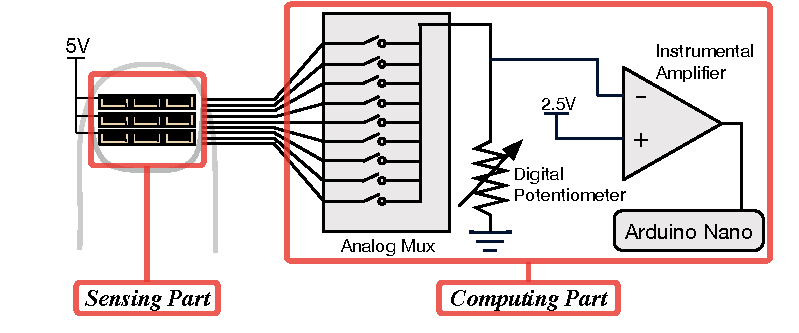
\includegraphics[width=1.1\columnwidth, height=0.47\linewidth]{figures/CompleteDiagram_v4.pdf}
  \caption{The complete circuit diagram. Sensing hardware consists of 9 strain gauges. Computing is performed by two analog multiplexers. The instrumental amplifier is made up of two amplifiers.}
  \label{fig:completeCircuitDiagram}
  \vspace{-0.8em}
\end{figure}

Since changes in voltage caused by strain are minuscule, two amplifiers are used to magnify the difference on both sides of Wheatstone bridge by a factor of 4000. The Arduino Nano reads the final analog value from the last amplifier's output. The digital potentiometer is used for adjusting the resistance when calibrating the Wheatstone bridge.

%\begin{figure*}[bp]
% \begin{center}
%  \setcounter{figure}{5}
%  \hspace{-1em}\includegraphics[width=2\columnwidth]{figures/mixedconfusingMatrix.pdf}
%  \caption{
%    Motionless mode: Confusing Matrix for each pressure level. Note that \textit{N} stands for Newton, \textit{P} stands for pitch and \textit{R} stands for roll.
%  }
%  \vspace{-1em}\label{fig:postureMatrix}
%  \end{center}
%\end{figure*}

% 可能的原因: (1)我們想要探討最基本的靜態的指甲變形,透過不同的角度會讓指甲變形來知道指甲在不同角度的分布情況?(但後面又沒有圖片佐證,很奇怪?)
% (2)
\section{System Evaluation}
First, we examined the reproducibility of strain on the fingernail (motionless mode). Then, we explored additional interaction techniques such as swipe gestures (motion mode).
The goals of our evaluation are as follows: (1) Reproducibility of strain values at different finger postures during typical usage at various pressure levels. (2) Capability of classifying different kinds of swipe gestures on surface.

In order to collect the typical pressure levels during daily usage, we conducted another user study with the same 10 participants from the prior pilot study. Participants performed tap gestures on an electronic load-cell allowing us to measure the pressure applied to its surface. The average of tap pressure measured 0.82N (SD=0.26).
%requested users to perform tap gesture on electronic load-cell to measure how much pressure is applied on a surface to investigate the ability of strain gauges.


\vspace{-0.4em}
\subsection{Participants}
We recruited 10 participants (6 male, 4 female) between the ages of 20 and 24 (mean 22.3). All participants were right-handed and used their right index finger to perform tap and swipe gestures for about an hour. All participants received \$5 in compensation for their time.


\begin{figure}[h!]
	\begin{center}
  \includegraphics[width=0.9\columnwidth]{figures/apparatus.pdf}
  \end{center}
  \caption{(a) Set-up of our user study. (b) A load-cell sensor below the surface measures pressure (c) A finger equipped with our \projectName{} device and a 9-DOF sensor.}
  \label{fig:apparatus}
%  \vspace{-1.3em}
\end{figure}

\vspace{-0.4em}
\subsection{Apparatus} %設備!
The apparatus is shown in \autoref{fig:apparatus}. We used the same load-cell sensor (error: $\pm 0.5$ grams) as used in our pilot study. In this experiment, we equipped the tip of the user's index finger with a 9 Degrees of Freedom (9-DOF) sensor. Since the strain gauges are very sensitive to outside forces, we avoided contact between the 9-DOF sensor and the fingernail, shifting it to the side of index finger as shown in \autoref{fig:apparatus}(c). The 9-DOF sensor is used exclusively to confirm that the user is performing the gesture at an allowed angle when collecting data. The surface we used during the experiment consisted of medium-density fibreboard. The board size was 18cm$\times$18cm and had a thickness of 3mm. 
% TODO 要把那個板子說的更明確一些, 確認大小 
%  which is a superior engineered wood used internationally in furniture construction.
\subsection{Task and Procedure}

\subsubsection{Motionless Mode}
During this experiment we collected strain gauge values for a variety of finger postures at different pressure levels.
For each trial, the participants were instructed to adjust their finger pitch and roll angles as shown in \autoref{fig:fingerposture} and then apply force onto the surface with a given force. A resting state posture was added for keeping the finger at the same initial position without touching the surface.
The forces were chosen based on our pilot user study: average force (0.8N), one SD forces (0.6N, 1.0N), two SD forces (0.4N, 1.2N). The participants were asked to straighten their finger during the entire experiment. A screen was placed in front of the user showing the current (based on 9-DOF and load-cell sensor) and instructed angle and force. Before each trial, participants were required to return to the resting state posture. When participants adjusted their finger to the correct posture and performed the correct pressure (tolerance: $\pm 5$grams), we started to collect data. We collected data for 5 postures at 5 force levels 5 times, resulting in a total of 125 trials for each user.

\subsubsection{Motion Mode}
We chose four swipe directions (up, down, left, right) and tap for this study.
Users were instructed to perform gestures shown on computer screen in front. On the surface, we drew a origin point and the end points for each direction to ensure swipe distance and angle are consistent. Swipe directions are randomly selected to show on screen, and collected with 10 sets of sequential data which contains a total of 50 trials for each user. A calibration is needed for the first time wearing but no further calibration was needed.


\begin{figure}[t!]
\setcounter{figure}{3}
  \includegraphics[width=1\columnwidth]{figures/fingerposture.pdf}
  \caption{Set of postures in motionless mode: (a) pitch 15 degrees, (b) pitch 45 degrees, (c) pitch 15 degrees and roll 45 degrees, (d) pitch 45 degrees and roll 45 degrees}
  \label{fig:fingerposture}
  	\vspace*{-2ex}
\end{figure}




\subsection{Results}
%\textit{Accuracy:} is defined as the number of correctly classified samples divided by the total number of samples.

\subsubsection{Gesture / Posture Recognition}
We used LIBSVM tool\cite{libsvm}, a popular machine learning open-source library for SVM, to distinguish the patterns by vectors.
Since each mode uses a different type of the input data sets, we implemented two algorithms specifically for finger postures (motionless mode) and swipe gestures (motion mode).
In motionless mode, raw data was directly used for machine learning.
In motion mode, sequential and time-based data was preprocessed by accumulating each datum's difference from the first received datum when the gesture began. At the end, the sequential data was processed to be represented by one feature datum.
For each mode, we normalized feature values to the range of -1 to 1 and then trained a multi-class SVM classifier with a Radial Basis Function (RBF) kernel.
\subsubsection{Motionless Mode}
The accuracy due to chance was 20\%. Off-line accuracy was computed using 5-fold cross-validation of the evaluation data. The mean accuracy for the forces data together across all participants was 76.9\% (SD: $\pm$13.17\%), and the confusion matrix is shown in \autoref{fig:postureResult}(a). 
Most error happened in the resting state and at angle of pitch 45 degrees with roll 45 degrees. When data collection was triggered at 0.4N and 0.6N of pressure, it was hard to distinguish the resting state from the other angle classes. For the angle, error was sometimes due to the user sometimes performing postures directly with the fingernail instead of the fingertip when the roll angle is higher. This caused strain gauges to have different values for each trial which raised the error in classification.
The accuracy for each force level is shown in \autoref{fig:postureResult}(b), which shows that at higher pressure levels the accuracy increased. If we remove data measured at pressure levels of 0.4N and 0.6N, accuracy increases to 82.44\% (SD: $\pm$12.74\%). 
%For sensing force touch, we used 5-fold cross-validation to evaluate. However, it shows that average can only distinguish 0.4N and 1.2N pressure with 70\% (SD: $\pm$12.74\%) accuracy.





% 此部分數據已確認!!
%\begin{figure}[t!]
%  \includegraphics[width=1\columnwidth]{figures/fingerposture.png}
%  \caption{Swipe Gestures in user study}
%  \label{fig:swipegestures}
%\end{figure}


\begin{figure}[hb!]
%	\begin{subfigure}{0.2\textwidth}
%	\hspace{-0.80em}\vspace{-0.3em}\includegraphics[width=1.05\linewidth, height=1.0\linewidth]{figures/overallConfusingMatrix.pdf} 
%%	\caption{Caption1}
%%	\label{fig:subim1}
%	\end{subfigure}
%	\begin{subfigure}{0.26\textwidth}
%	\vspace*{1ex}\includegraphics[width=1.0\linewidth, height=0.7\linewidth]{figures/postureAcc.pdf}
%
%%	\caption{Caption 2}
%%	\label{fig:subim2}
%	\end{subfigure}
	\includegraphics[width=1\columnwidth]{figures/postureMerge.pdf}	 
%	\caption{Caption for this figure with two images}
%	\label{fig:image2}


%  \includegraphics[width=1\columnwidth]{figures/swipeconfusing.pdf}
  \caption{Motionless mode: (a) Mixed-force confusion matrix (b) Accuracy for each level of pressure.}
  \label{fig:postureResult}
  \vspace*{-2ex}
\end{figure}

\begin{figure}[hb]
%swipeMerge
\includegraphics[width=1\columnwidth]{figures/swipeMerge.pdf}	 
%	\begin{subfigure}{0.2\textwidth}
%	\hspace{-0.5em}\includegraphics[width=1.02\linewidth, height=1.0\linewidth]{figures/swipeconfusing.pdf} 
%%	\caption{Caption1}
%%	\label{fig:subim1}
%	\end{subfigure}
%	\begin{subfigure}{0.26\textwidth}
%	\vspace*{1ex}\includegraphics[width=1.0\linewidth, height=0.8\linewidth]{figures/swipeAcc.pdf}
%
%%	\caption{Caption 2}
%%	\label{fig:subim2}
%	\end{subfigure}
	 
%	\caption{Caption for this figure with two images}
%	\label{fig:image2}

%  \includegraphics[width=1\columnwidth]{figures/swipeconfusing.pdf}
  \caption{Motion mode: (a) Confusion matrix (b) Accuracy for the four directions swiping and tapping. }
  \label{fig:swiperesult}
  \vspace*{-0.5em}
\end{figure}
The mixed-force leave-one-user-out accuracy was computed, which was low at an average of 55.2\%(SD: $\pm 13.6$\%).

\subsubsection{Motion Mode}
The result of this study is shown in \autoref{fig:swiperesult}. Off-line accuracy was computed using 10-fold cross-validation of the evaluation data. The mean accuracy across all participants was 93.2\%(SD: $\pm 5.98$\%). Most of the error occurred during swipe down and up gestures, likely due to the higher friction causing users to  perform gestures lightly on the surface which caused strains on fingernail to become less observable for the sensor. Leave-one-user-out was also computed, and the accuracy was 44.2\%(SD: $\pm 12.9$\%) which indicates strains had significant difference between participants.


\vspace{-0.2em}
\section{Example Application}
Based on the advantage of \projectName{}, we describe two examples using this new sensing technique and are included in video.

\vspace{-0.2em}
\subsection{Controlling Smart TV / Devices}
% TODO Device
Smart TV's require us a remote for controlling. With \projectName{}, users can focus on the TV program without a remote. Users can use a desk or nearby surfaces as an input surface to perform simple tap and swipe gestures for switching channels and selection. Furthermore, we also implemented this on smart watch. Due to the smaller screen, a swipe gesture on the surface is a simple interaction method.

\vspace{-0.2em}
\subsection{Short cuts within application}
For touchscreens, most devices can only be distinguished by a binary state of touch. Using \projectName{}, the user can use different finger posture to enable shortcuts such as right clicking on computer mouse. For instance, the file system on a smart phone can be controlled with 45 degree of roll angle to show a drop-down list to delete, move, and change the file name.

\vspace{-0.2em}
\section{Limitation and Future Work}
\textit{Firmly adhering sticker to fingernail:} In our evaluation of system, we noticed that the artificial-skin lost adhesiveness over time and after many times of usage. This caused misclassifications due to the sensing part becoming detached. We will continue to find another option for device adhesion.
% TODO How many time?

\textit{Minimize computing part and power consumption:} As shown in \autoref{fig:main}, we currently put the computing part on the wrist as a wristband form factor. The form factor is determined by the Arduino Nano board size. This motivates us to minimize the computing part into a ring form factor in future studies. For power consumption, we currently use 120-ohm strain gauges which can be replaced by much higher ohm gauges. 
% TODO check power consumption?

\textit{Force touch and sensing from all fingers:} Since currently we only examined the daily usage pressure level, the higher force will be our future work to explore the device's force sensing. Moreover, mounting the device on all our fingernails will also be researched in our future work for multi-touch input such as pinch and zooming.

% TODO 可以討論多一點

\section{Conclusion}
In this paper, we evaluated using strain on fingernail as a input technique. We developed a nail-mounted device called \projectName{}, which is light and small enough to fit on top of fingernails. Evaluation of the this technique shows that \projectName{} can distinguish finger postures on surface at average force level with 82.22\% accuracy. Furthermore, swiping directions can be identified at high accuracy (93.2\%). The system is also attractive for a nail-mounted readily available input for surfaces nearby which enrich the mobility of touch interaction. Our currently plans are to sense force touch and extend this system to all fingers for enabling multi-touch input.
%Evaluation of the this shows that it can distinguish swipe gestures on surface in high accuracy (93.2\%). Not only for swiping but also the finger postures can identify five different kinds of finger posture at average force level with 82.22\% accuracy.
% TODO 已刪除用senario結尾很奇怪 但還是需要改嗎?

% \subsection{Title and Authors}
% \subsubsection{Sub-subsections}
% $\times$
% \texttt{.cls}

%%%

% Use a numbered list of references at the end of the article, ordered
% alphabetically by first author, and referenced by numbers in
% brackets~\cite{ethics, Klemmer:2002:WSC:503376.503378,
%   Mather:2000:MUT, Zellweger:2001:FAO:504216.504224}. For papers from
% conference proceedings, include the title of the paper and an
% abbreviated name of the conference (e.g., for Interact 2003
% proceedings, use \textit{Proc. Interact 2003}). Do not include the
% location of the conference or the exact date; do include the page
% numbers if available. See the examples of citations at the end of this
% document. Within this template file, use the \texttt{References} style
% for the text of your citation.

% Your references should be published materials accessible to the
% public.  Internal technical reports may be cited only if they are
% easily accessible (i.e., you provide the address for obtaining the
% report within your citation) and may be obtained by any reader for a
% nominal fee.  Proprietary information may not be cited. Private
% communications should be acknowledged in the main text, not referenced
% (e.g., ``[Robertson, personal communication]'').
%
%\begin{table}
%  \centering
%  \begin{tabular}{r c c}
%    \toprule
%    & \multicolumn{2}{c}{\small{\textbf{Caption}}} \\
%    \cmidrule(r){2-3}
%    {\small\textbf{Objects}}
%    & {\small \textit{Pre-2002}}
%    & {\small \textit{Current}} \\
%    \midrule
%    Tables & Above & Below \\
%    Figures & Below & Below \\
%    \bottomrule
%  \end{tabular}
%  \caption{Table captions should be placed below the table. We
%    recommend table lines be 1 point, 25\% black. Minimize use of
%    unnecessary table lines.}~\label{tab:table1}
%\end{table}

%\begin{figure*}
%  \centering
%  \includegraphics[width=2\columnwidth]{figures/map}
%  \caption{In this image, the map maximizes use of space. You can make
%    figures as wide as you need, up to a maximum of the full width of
%    both columns. Note that \LaTeX\ tends to render large figures on a
%    dedicated page. Image: \ccbynd~ayman on
%    Flickr.}~\label{fig:figure2}
%\end{figure*}

% \begin{itemize}
% \item text
% \end{itemize}
% \ref{tab:table1}

% \begin{enumerate}
% \item text
% \end{enumerate}


%\section{Acknowledgments}
%
%Sample text: We thank all the volunteers, and all publications support
%and staff, who wrote and provided helpful comments on previous
%versions of this document. Authors 1, 2, and 3 gratefully acknowledge
%the grant from NSF (\#1234--2012--ABC). \textit{This whole paragraph is
%  just an example.}

% Balancing columns in a ref list is a bit of a pain because you
% either use a hack like flushend or balance, or manually insert
% a column break.  http://www.tex.ac.uk/cgi-bin/texfaq2html?label=balance
% multicols doesn't work because we're already in two-column mode,
% and flushend isn't awesome, so I choose balance.  See this
% for more info: http://cs.brown.edu/system/software/latex/doc/balance.pdf
%
% Note that in a perfect world balance wants to be in the first
% column of the last page.
%
% If balance doesn't work for you, you can remove that and
% hard-code a column break into the bbl file right before you
% submit:
%
% http://stackoverflow.com/questions/2149854/how-to-manually-equalize-columns-
% in-an-ieee-paper-if-using-bibtex
%
% Or, just remove \balance and give up on balancing the last page.
%
\balance{}


% REFERENCES FORMAT
% References must be the same font size as other body text.
\bibliographystyle{SIGCHI-Reference-Format}
\bibliography{sample}

\end{document}

%%% Local Variables:
%%% mode: latex
%%% TeX-master: t
%%% End: